\chapter{Volunteer computing}
% Pu these two ines after every \chapter{} command
\vspace{-2em}
\minitoc

The basic concepts of distributed and volunteer computing are reviewed in this chapter.  A brief historical overview   of some popular distributed and volunteer projects is also provided.  \emph{Berkeley Open Infrastructure for Network Computing} (BOINC), in particular,  is examined in some detail, starting with basic concepts and the steps required to create a volunteer computing project. Some consideration is also given to special types of applications and the requirements of setting up a BOINC server, as well as common security concerns and challenges facing distributed and volunteer project administrators.  
 
\section{A historical overview of public-resource computing} \label{VChist}
In John Brunner's 1975 science-fiction novel, \emph{The Shockwave Rider} \cite{brunner}, the main character creates a ``tapeworm" program which is able to propagate itself through a network of computers, replicating when needed and consuming resources wherever available. This type of program, capable of harnessing resources on any number of machines, piqued the interest of a group of researchers at Xerox's Palo Alto Research Center (famously the home of the first graphical user interface) which set about creating a number of ``worms"   for controlling multi-machine performance measurements of their pioneering first Ethernet network \cite{worms}. 
Distributed computing systems  were mainly confined to networks within organisations or academic departments for the following two decades.
An early example  of such a distributed computing system is \emph{HTCondor} \cite{condor, condor1}. This system was was developed in 1988 and was originally known as \emph{Condor}, and is still active today.
The recent widespread public adoption of personal computers and the internet has, however,  made it possible to involve the public in distributed computing, also known as \emph{volunteer computing}.

Anderson \emph{et al.} \cite{boincwiki} define volunteer computing as a form of computing where both organizations and members of the public can donate unused computing resources to computing projects, which are usually applications of a scientific or academic nature. Volunteer computing is built largely on trust and mutual goodwill as it is necessary that the volunteers trust the projects not to perform unapproved calculations using their resources and to guard their personal account details carefully. Similarly, although IP and email addresses may be linked to individual volunteers, volunteers remain largely anonymous and no disciplinary steps are typically available to curb   volunteers who wilfully corrupt computations. For project administrators the main advantages of volunteer computing are, firstly, that it provides access to at least part of the approximately 10 billion devices linked to the internet \cite{anderson2013,cisco} and, secondly, that it raises public awareness of scientific endeavours and provides a mechanism through which a project of large popular appeal, but little funding, may flourish \cite{boincwiki}. Volunteers, on the other hand, are able to contribute to scientific projects which interest them and are rewarded in credits, which become somewhat of a status symbol.

Volunteer computing is somewhat similar to two other forms of distributed computing, namely \emph{grid computing} and \emph{peer-to-peer} networks. Grid computing is generally considered a paradigm through which computing resources are shared within and between organizations in a mutually beneficial way. An example of such a system is a   desktop grid consisting of  all the desktop computers within an organization. Grid computing has many aspects in common with volunteer computing, but differs in that the ``volunteers" are usually more reliable because of a lack of anonymity and the accompanying existence of disciplinary measures \cite{fostergrid,boincwiki}. The principles of peer-to-peer computing, on the other hand, is  perhaps best seen in file-sharing services such as \emph{Napster} \cite{napster} or \emph{BitTorrent}   \cite{bittorrent} --- data transfer takes place between computers without any form of coordination by central servers \cite{peer, peer2}. Volunteer computing relies on central servers hosting the project and it is not possible for two clients to communicate directly in such a computing paradigm without coordination by the central servers.  

There are, however, also many challenges associated with publicly distributed computing. For example, the platforms on which   applications must be able to execute accurately have become rather more heterogeneous  and a distributed computing   network is likely to be much more unreliable than  a computer network within a corporation or laboratory.   Despite these factors, scientists have become increasingly interested in unlocking   the massive computing power which   lies dormant in the idle computer cycles of the public. Two early volunteer computing projects, the \emph{Great Internet Mersenne Prime Search} (GIMPS), which searches for very large Mersenne primes \cite{gimps}, and \emph{distributed.net} \cite{distnet}, which facilitates brute-force decryption, were created in 1996 and 1997, respectively. 

GIMPS is still active today and currently runs on more than $730\,000$ CPUs around the world, with an average annual throughput close to  130 TFLOPs\footnote{1 TeraFLOPS of computing power is equivalent to $10^{12}$ floating point operations per second} \cite{gimps}. Mersenne primes of the form $2^n-1$, for integer  values of $n$, account for most of the very large prime numbers known today. The first Mersenne prime discovered by GIMPS, namely $2^{1\,398\,269}-1$, was found in November 1996 \cite{hayes}, while the  forty-eighth Mersenne prime, and the currently largest known prime number, namely $2^{57\,885\,161} -1$, was   found on 25 January 2013 \cite{gimps}. 
The network \emph{distributed.net} also remains active   and concerns itself with finding optimal Golomb rulers (combinatorial curiosities with application to the placement of radio antennas in astronomy) and deciphering encoded messages \cite{distnet}, a trend which, according to Hayes \cite{hayes}, started when the company RSA Data Security  issued a number of challenges in 1997, hoping to test how easily their encryption systems were breakable and to demonstrate the inefficiencies of rival schemes. Notable early successes were the breaking of RSA-129, which involved the factoring of a 129-digit number   and  took 600 volunteers eight months to perform, and the decryption of a message encrypted using the \emph{Data Encryption Standard} (DES), which was developed under US government sponsorship in the 1970s \cite{distnet}. 
Another early project, which has grown into one of the most influential volunteer computing projects, is  \emph{SETI@Home} (an abbreviation for \emph{Search for Extraterrestrial Intelligence}), launched  in 1999 by a group of scientists from the University of California at Berkeley to examine radio waves detected by a telescope operated by Cornell University and the National Science Foundation in Arecibo, Puerto Rico \cite{anderson:seti2002}. The project was very well received by the public and attracted millions of volunteers, by 2004 the average sustained processing power of the SETI@Home project was more than 70 TeraFLOPs, more than double the 35 TeraFLOPs of the most powerful supercomputer at that stage, the NEC Earth Simulator \cite{anderson2004boinc}.
 
According to Anderson \emph{et al.\ }\cite{anderson:seti2002}, the encouraging success of these early projects led to  wider support for frameworks which could be used for public-resource or large-scale distributed computing. In 1999, the \emph{Global Grid Forum} was formed as an umbrella corporation for a number of distributed projects, collectively called \emph{The Grid} \cite{fostergrid}, for resource sharing amongst research organizations, while many private organizations, including \emph{Platform Computing} and \emph{United Devices}, were developing corporate systems for distributed storage and computing. A number of middleware systems were launched including \emph{Sun Grid Engine} in 2001 \cite{oracle} (now called the \emph{Oracle Grid Engine}), \emph{Advanced Resource Connector} in 2002 \cite{arc} and the \emph{Globus} toolkit in 2004 \cite{globus}. BOINC was also launched in 2004 \cite{anderson2004boinc}, spearheaded by David Anderson, who was the Chief Science Officer   at United Devices at the time and also co-founder of the SETI@Home volunteer computing project. 

More than 80\% of the currently active public-resource computing projects make use of BOINC and, as such, it is the focus in the remainder of this chapter as an example of a middleware framework for distributed computing. BOINC (and other middleware) provides simple interfaces for both volunteers and scientists, and handles the required network connections automatically, thereby considerably decreasing the difficulty of establishing a new project. It also  provides scientists with a comprehensive \emph{Application Programming Interface} (API) with which to interact with volunteers and to enable volunteers to use the same client to connect to multiple volunteer computing projects. The first project to make use of BOINC was, unsurprisingly, SETI@Home. A large number of scientific projects followed suit with applications ranging from testing Einstein's theory of general relativity (\emph{Einstein@Home}) \cite{eah} and finding new arrangements into which proteins may fold themselves (\emph{Folding@Home}) \cite{fah} to the distributed rendering of animated films (\emph{BURP}) \cite{burp}.
A number of large organizations are also  engaged in volunteer computing through BOINC, for example,    IBM through their \emph{World Community Grid} (WCG) initiative which serves the community by computing vaccines for malaria and modelling the earth's fresh-water supply \cite{wcg}, CERN, which uses the \emph{LHC@Home} project to process  vast quantities of data obtained from experiments in their {Large Hadron Collider} \cite{lhcah}, and Oxford University in the UK, which  runs a number of different models estimating the effects of climate change on \emph{Climateprediction.net} \cite{cpdn}.  

BOINC remains under active development by a group of software developers and project administrators. A BOINC client for Google's open-source mobile operating system \emph{Android} has recently been released, thereby enabling the approximately 470 million Android smartphones in the market \cite{mobithinking}, many of which have two, four or even eight processors,      to take part in volunteer computing \cite{android}.
\section{The Berkeley Open Infrastructure for Network Computing} \label{Boincgen}
The main aim of BOINC is to simplify setting up a large-scale volunteer computing project, to minimize the time required for administrating the day-to-day running of the project and to enable a single computer, after a few weeks of work, to perform the role of a server for a project involving thousands of volunteers. Reducing the entry cost to volunteer computing has enabled many scientists with widely varying backgrounds and only moderate programming skills to take advantage of public resources for their computing endeavours, something which would not have been possible had it been necessary that they design the entire system themselves. According to Anderson \cite{anderson2004boinc},  secondary design goals included support for a diverse set of applications and programming languages, allowing for the sharing of resources between autonomous projects by letting volunteers simultaneously take part in a number of projects by assigning a priority to each project   and, finally, rewarding the volunteers in some way by measuring their  contributed resources.

As enticing as  the advantages of public resource computing and BOINC, in particular, may seem, it is important to note that not all applications   work equally well within this model. For a project to be successful in  utilizing public resources, especially in the developing world where high-speed internet is still a rarity,  it is firstly  very important that the application  should have a large computation to data ratio (so that small data transfers to volunteers can lead to multiple hours of computations) and, secondly, that the execution of the application should be independently parallelisable. Some classes of applications which seem particularly well suited to this type of distribution are described in \cite{anderson:pc}. An example of such an application is the simulation of   physical systems  in which every simulation is independent of the others  or physical models in which complex parameter spaces which must be explored. Random and genetic algorithms may also benefit from volunteer computing, as every independent trail can be performed by a different volunteer in the case of random algorithms, while for genetic algorithms every volunteer may receive an initial population of solutions to  evolve from independently. A final category of projects, which has perhaps proven most successful in practice, involves the analysis of large amounts of data, such as from radio telescopes (as in the case of SETI@Home) or  from the Large Hadron Collider (as in the case of LHC@Home) \cite{anderson:pc}.

 \subsection{Basic workflow and concepts of volunteer computing} \label{Bconcepts}
According to \cite{boincwiki}, a BOINC \emph{project} is a self-contained entity consisting of a  database, website, \emph{applications}, \emph{work units} and \emph{results}.

An application consists of a number of different executable programs, usually one for every \emph{platform} on which the project is  available. Standard platforms are pre-defined in BOINC and are   combinations of CPU architectures and operating systems (\emph{e.g.\ }a 32-bit Intel processor running Windows or a 64-bit Intel processor running Linux). Knowing on which platform a computation is performed  is important for ensuring correct results, as different platforms handle floating-point operations in different ways and this may lead to discrepancies in results if ignored.

A work unit is a computation that has to be performed. It is associated with a specific application and has various attributes, including the names of its input files, the estimated execution time, and the resources required to complete it. As was mentioned in \S\ref{VChist},   the results returned by volunteers may not necessarily be trustworthy. Volunteer computing projects usually mitigate this risk through \emph{redundant computing}, which means that every work unit is computed multiple times by different volunteer and the results are compared for correctness. A \emph{result} may therefore be seen as a copy of a work unit which is sent to a volunteer for computation.  Once a certain number, called a \emph{quorum}, of results of a specific work unit have been returned, they are compared to find the definitive or \emph{canonical} result for that work unit.


All workunits and results are stored in a database on the server, along with additional information regarding applications, workunits, volunteers and hosts. A distinction is made between a volunteer, who creates an account with an email address and password when joining a project, and a host, which is the actual machine performing the computation. A single account may thus have a number of hosts associated with it, each running a version of the BOINC client which allows the host to attach to scientific projects. Some measure of credit is associated with an account, so that all hosts running under the same account earn credit in the same place.

Once a volunteer host has  connected to a specific project through the client it may request work from the project's servers. 
A deamon (a small, periodically executed task-specific program) running on the server,  called the \emph{scheduler}, takes the host's resources into account and dispatches suitable results, if any are available, after which the computation takes place on the host. 
Once the computation has been completed the client on the host will  report the results to the server along with a   request for further work. 
The   results thus received are stored on the server until their respective quorums are met, after which the results are tested for correctness, a process called \emph{validation},   credit is assigned to correct results and the results are finally processed or \emph{assimilated}. 
In the meantime, the host would have received new results for processing and the process, as illustrated in Figure \ref{fig:workflow}, may be repeated as long as there are uncompleted results available.
\begin{figure}[htb]
\centering
\includegraphics[width=14cm]{images/boincwork}
\caption{The basic workflow on the client and BOINC project server.}\label{fig:workflow}\vspace{-.2cm}
\end{figure}
\subsection{Grid-enabling a simple BOINC project} \label{Bgridenable}
A scientist attempting to turn an existing application into a volunteer computing project must  determine how the application will be parallelised, modify the existing application to make use of the BOINC API and finally provide the server-side deamons responsible for scheduling,  generating new workunits and validating and assimilating incoming results.
The first of these tasks, parrellelising the computation, is highly application-specific and has little to do with the structure and components of a BOINC project, but it may be insightful to give further consideration to the BOINC API and the various deamons running on the server.
\subsubsection{The BOINC API} \label{Bapi}

The BOINC API provides a set of functions that   allow the client and the application to communicate and   improves portability of the application between different platforms.
An application must notify the client when it initialises through a call to \verb|boinc_init| and return a value when terminating so that the client may track whether the computation was successful or not. 
The API also handles input and output, resolving logical names to actual file names as specified in the workunit and providing wrappers for functions which execute differently on different platforms. An example of such a wrapper occurs in the  \verb|boinc_fopen| function which replaces the standard \texttt{fopen} call for opening functions so that on Windows hosts, where files may become temporarily locked, the function attempts to open the file multiple times within short succession while on Unix, where \texttt{fopen} occasionally fails with a specific error code, it tests for this error code and retries accordingly. 

\emph{Checkpointing}, or saving the current state of the computation in such a way that the computation may be resumed from that point, is very important in volunteer computing as there is no way of knowing when a host may be turned off or fail. Applications may choose their own minimum time between checkpoints, usually based on how long it takes to checkpoint, and may repeatedly call the function \verb|boinc_time_to_checkpoint| to determine when to checkpoint. Checkpointing is also an example of a \emph{critical section} of an application,   which may not be interrupted by the client.
\begin{table}[htb] \centering
\caption{The core of the BOINC C/C++ API \cite{boincwiki}.}
\begin{tabular}{p{2.5cm}p{11.6cm}}\toprule
 API method & Description\\ \cmidrule(r){1-2}
 \verb|int boinc_init()|\\ & The call that notifies the client that a computation has begun.\\
\verb|boinc_cpu_time()| \\ & The CPU time that the current computation has taken.\\
\verb|int boinc_finish(int status)| \\ & The call that notifies the client that a computation has been completed, along with its exit status --- 0 if successful or some integer error code.\\
\verb|int boinc_resolve_filename(char *logical_name, char *physical_name)| \\ & Converts logical file names, such as `in,' used in the application to physical   file names. \\ 
\verb|bool boinc_time_to_checkpoint()| \\ & Tests whether it is time for the application to checkpoint.\\
\verb|void boinc_checkpoint_completed()| \\ & Notifies the client that a checkpoint has been completed, the countdown timer for checkpointing must be reset and that the program is exiting a critical section. 
\\ 
\verb|boinc_fraction_done(double fraction_done)| \\ & Reports the current progress to the client. \\ 
\verb|void boinc_child_start()| \\ & Notifies the client that the main program has started a subsidiary thread.\\
\verb|void boinc_child_done(double total_cpu)| \\ & Notifies the client that   a subsidiary thread has been completed. 
\\ \bottomrule
\end{tabular}\label{tab:api}
\end{table}
 
BOINC  allows communication between the application and server through \emph{trickle messages}, which are small messages that are sent up from the client or down from the server and which are assigned a very high priority. A trickle down message may, for example, be sent to notify an application that the result which it is computing is no longer needed and should be aborted. Similarly a trickle-up message may be sent to the server to notify it that, although a result  has exceeded its deadline, it is still being successfully computed, in which case the original deadline should be extended.
The remainder of the API mainly focusses on providing methods which allow the client  to register the time that a computation takes and monitor its progress. The full API, along with a brief summary of every function as described in \cite{boincwiki}, may be found in Table~\ref{tab:api}.


 
\subsubsection{Deamons} \label{Bdeamons}
The main task of the work generator is inserting new work units or jobs into the project database. This may happen once, at the start of the project, in a number of discrete batches or continuously as results are returned by volunteers. It is also possible to develop a web interface which allows for the remote submission of jobs.
Before implementing the work generator, however, project managers must decide on templates for the work units and results. These templates are \emph{XML} (extensible markup language) files which provide  the application with the necessary information for performing a work unit and are typically re-used for millions of jobs. 
An input template may, for example, specify the name of the actual file to which the logical file name must be resolved, possible command-line arguments along with work unit attributes such as an estimate of its execution time, the resources required for the computation and the deadline by which the server expects to receive the result before re-issuing the work unit to a different host.  
Similarly, the output template defines the number of files returned to the server and where they may be located  or generated. A selection of the most important options that may be specified in the input and output templates may be found in Tables \ref{tab:intemplate} and \ref{tab:outtemplate}, respectively. The work generator ensures that the required files and templates are available before entering the work unit into the database, either through a command-line tool or  a C/C++ method which is part of the BOINC API.
\begin{table} 
\caption{A selection of the parameters that may be specified in the input template of BOINC \cite{boincwiki}. }
\begin{tabular}{lp{11.5cm}}\toprule
Work unit attributes & Description \cite{boincwiki} \\ \cmidrule(r){1-2}
\verb|open_name| & The logical name of the file used in the application, \emph{e.g.\ `in'}.\\
\verb|command_line| & The command-line arguments to be passed to the main  application.  \\
\verb|rsc_fpops_est| &
An estimate of the number of floating point operations required to complete a job, used to estimate how long the job will take on a given host.\\
\verb|rsc_fpops_bound| &
An upper bound on the number of floating point operations required to complete a job. If this bound is exceeded, the job will be aborted.\\
\verb|rsc_memory_bound| &
An estimate of a job's largest working set size. A job is only sent to hosts with at least this much available RAM. If this bound is exceeded, the job is aborted.\\
\verb|rsc_disk_bound| &
A bound on the maximum disk space used by a job, including all input, temporary, and output files. The job is only   sent to hosts with at least this much available disk space. If this bound is exceeded, the job is aborted.\\
\verb|rsc_bandwidth_bound| &
If non-zero, a job is sent only to hosts with at least this much download bandwidth. Mainly used for jobs with very large input files. \\
\verb|delay_bound| &An upper bound on the time (in seconds) between sending a result to a client and receiving a reply.  If the client does not respond within this interval, the server `gives up' on the result and generates a new result, to be assigned to another client.  
\\
\verb|min_quorum| &
The minimum size of a quorum. The validator is run when there are this many successful results. If a strict majority agrees, the result is considered correct. This value is set to two or more if redundant computing is required.
\\
\verb|target_nresults| &
How many results to create initially. This must be at least \verb|min_quorum|. It may be more in order to reflect the ratio of result loss, or to get a quorum more quickly.
\\
\verb|max_error_results| &
If the number of client error results exceeds this value, the work unit is declared to contain an error; no further results are issued, and the assimilator is triggered. This safeguards against work units that cause the application to crash.
\\
\verb|max_total_results| & If the total number of results for this work unit   exceeds this value, the work unit is declared to be in error. This safeguards against work units that are never reported (\emph{e.g.} because they crash the core client).
\\
\verb|max_success_results| & If the number of successful results for this work unit exceeds this value, and a consensus has not been reached, the work unit is declared to be in error. This safeguards against work units that produce non-deterministic results.
\\
\verb|priority| &  Higher-priority work units are dispatched first. \\
\verb|size_class| & Used to define work units of different sizes, for example in the case where the GPU version of an application is orders of magnitudes faster than the CPU version. \\ \bottomrule
\end{tabular} \label{tab:intemplate}
\end{table}

\begin{table} 
\caption{A selection of the parameters that may be specified in the output template of BOINC \cite{boincwiki}.}
\begin{tabular}{lp{11.6cm}}\toprule
Output attributes & Description \cite{boincwiki}    \\ \cmidrule(r){1-2}
 \verb|name| & The physical file name of the output file\\
\verb|open_name| & The ``logical name" by which the application will reference the file.\\
\verb|max_nbytes| & Maximum file size. If the actual size exceeds this, the file will not be uploaded, and the job will be marked as an error.\\
\verb|url| & The URL of the file upload handler. \\ 
\verb|no_delete| & If present, the file will not be deleted on the server even after the job is finished.\\
\verb|report_immediately| & If present, clients will report this job immediately after the output files are uploaded, otherwise they may wait up to a day. 
\\  \bottomrule
\end{tabular}\label{tab:outtemplate}
\end{table}

It is highly likely that a new project will, at least initially, make use of the default scheduler  provided along  with the BOINC source code.
The scheduler is  mainly responsible for dispatching new versions of applications, accepting requests for work from hosts and assigning work to hosts based on a combination of their available resources, the estimated execution time of the available work units and the historical accuracy of a host. Larger work units are thus preferably sent to hosts who have  historically returned fewer erroneous results and who have more resources available in order to minimise the expected computation time that will be wasted if a host returns an error after an extended period of   work.
Secondary objectives which may be included in the scheduler are completing a specific batch of work units as soon as possible and limiting the number of work units that a host may receive on a single day (so as to prevent hosts from repeatedly returning the same results and claiming credit for them).

The main task of the validator is to compare results for correctness. Care should be taken when comparing results from different platforms --- for example, the end-of-line character is different between Windows and Linux, making a character-by-character comparison of the output files impossible. If an application performs many floating-point operations, projects  may elect to enforce a measure called \emph{homogeneous redundancy} to ensure that results from the same work unit are assigned to identical platforms. Alternatively,  ``fuzzy" comparisons may be made by comparing floating-point numbers with a degree of tolerance \cite{boincwiki}. A measure called \emph{adaptive replication} may also be used, which dynamically determines the number of replications of a specific work unit based on the historical error rate of the host which was assigned the first result --- if the host usually returns accurate results, the probability of replication taking place for that work unit will be small.
Validation takes place by majority once a quorum of results has been received and marks a result, along with its associated output files, as the canonical result against which any other results of the same work unit are compared in order to determine whether it was computed successfully and deserves credit.
Two sample validators are provided with the BOINC source code: the first is mainly used for testing purposes and simply marks every received result as successful, while the second performs a bitwise comparison of output files.

Once results are verified, they should be marked accordingly in the database so that they are not assigned to any further hosts. The input files of verified results may be deleted from the location where they were accessible to hosts and the canonical output files may be moved to a specific location.
The sample assimilator does exactly this and it is up to project administrators to decide which other post-processing tasks to perform on validated results.

Projects that use   trickle messages must also provide a deamon to handle these messages. Trickle messages may, for example, be used by the application to  send its current computation state to the server periodically  so that the server may   determine whether to assign partial credit for the work done up to the current point  or   to abort the computation based on some internal logic.

The most important interactions in a BOINC project are illustrated in Figure \ref{fig:server}. Note that the transitioner and file deleter are responsible for generating new results if invalid or erroneous results are received and deleting the input files of fully completed workunits, respectively, but have not been discussed since the default versions suffice.
\begin{figure}[htb]
\centering
\includegraphics[width=12cm]{images/boincserver}
%\input{images/boincserver.pdf_t}
\caption{An example of the server setup showing the interaction of the MySQL database with the BOINC clients and various server deamons.}\label{fig:server}\vspace{-.2cm}
\end{figure}

\subsection{Special types of applications} \label{Btypes}
In addition to the basic functionality described in the previous section, BOINC allows applications to display graphics, execute on multiple cores or GPUs through OpenCL \cite{opencl}  and CUDA \cite{cuda}, or even to run entirely within a virtual machine. 
\subsubsection{Graphics applications} \label{Bgraphics}
Publicly-launched volunteer computing projects usually attempt to provide volunteers with some visualisation of the computation running on their machines, either as   screensavers or in   windows which can be opened in the BOINC Client Manager. The main reason for providing graphics is to further engage the public in the goals of and progress made in a scientific project in order to increase involvement. Examples of graphics provided by SETI@Home and WCG may be seen in Figure \ref{fig:boincgraphics}.
\begin{figure}[htb]
\centering
\begin{minipage}{7.5cm}
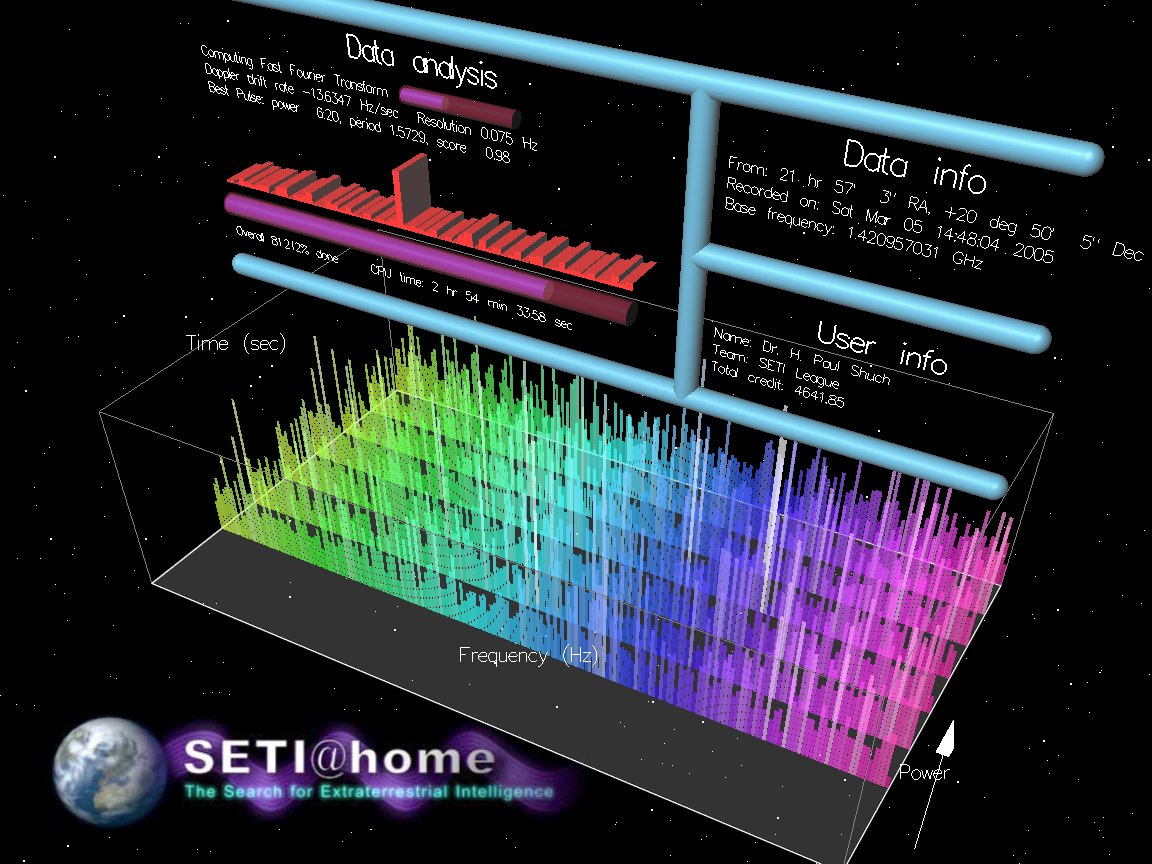
\includegraphics[width=7.5cm]{images/graphics1}
 \end{minipage} \hspace{.1cm}
\begin{minipage}{7.5cm}
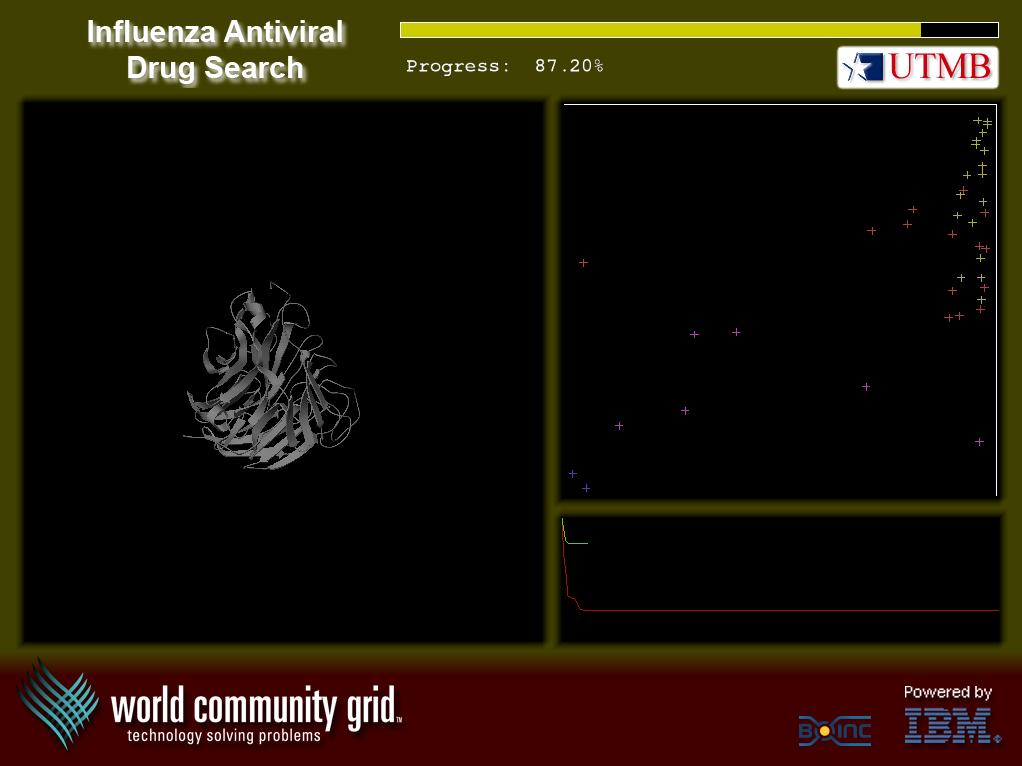
\includegraphics[width=7.5cm]{images/graphics2}
 \end{minipage}
\caption{Graphical applications in SETI@Home and WCG provide volunteers with an indication of the state of the current computation.} \label{fig:boincgraphics} 
\end{figure}

  In a  recent survey of $15\,627$ volunteers by IBM's World Community Grid project \cite{wcg}, however, 72\% of volunteers stated that they either disabled the graphics or did not pay attention to it  \cite{wcg2013}, thereby casting some doubt on the actual benefit of graphical applications. Graphics applications are usually separate from the main scientific application, built on  a specific  BOINC graphics library and make  use of OpenGL \cite{opengl}. Communication with the main application takes place through shared memory --- the main application would periodically store a representation of its current state and progress in  a block of memory which is accessible to the graphics application, from where it is read and displayed. Graphics applications can also display static images, text or web-based graphics by opening   browser windows pointing to   specific URLs.

\subsubsection{Muti-core and GPU applications} \label{Bopencl}
CPU manufacturers have been dealing with the limit placed on CPU frequency by increasing the number of cores provided and it seems that this trend will continue in the foreseeable future \cite{spu}. In cases where the completion time of individual work units have to be improved, or the memory footprint of the application is too large to allow a separate copy of the application to run on every core, it may be desirable to implement a multi-threaded application developed in OpenCL, MPI \cite{mpi}, OpenMP \cite{openMP}, CUDA  or a number of other languages. BOINC also supports what it calls `coprocessors,' or GPUs, designed by NVIDIA, AMD or Intel. Available GPUs are reported to the scheduler by the BOINC client, which also keeps track of which instances are currently allocated on every GPU. To prevent system failures, GPU kernels are  executed within critical sections, which may not be killed by the BOINC client and  BOINC projects may define work units of different size classes to compensate for the potentially dramatic difference in speed between CPU and GPU versions of the same applications,  thereby ensuring that a typical work unit will take approximately the same amount of time irrespective of the architecture on which it is executed.

\subsubsection{Applications which run inside virtual machines} \label{Bvmach}
BOINC supports applications which run entirely within virtual machines. This approach has two distinct advantages in that it provides the highest level of security for the host machine, as virtual machines cannot access or modify the host system, and there is no need to build applications for different architectures, as every application will run on a virtual computer with exactly the same runtime environment on all platforms.  
There are, however, also some additional complexities that arise from using applications inside virtual machines, such as the fact  that hosts require software such as VirtualBox to mount the machine image, yet VirtualBox  is not currently available for all processors. Furthermore, GPU applications cannot currently run inside VirtualBox and not all processors are capable of running both 32- and 64-bit virtual machines, so images of both architectures   have to be provided. Distributing the virtual machine image also increases the size of the first download to approximately 200Mb, which may be prohibitive for volunteers with limited bandwidth.

\subsection{Setting up a server and project maintenance} \label{Bserver}
As described in \S \ref{Bconcepts},   a BOINC project consists mainly of a MySQL database, a directory structure and a configuration file which specifies the options, deamons and periodic tasks that must be performed and, as such, it is possible to use almost any computer as a  BOINC server \cite{boincwiki}.

Since   reliability and security are of the utmost importance, a server should have a static IP address and at the very least be placed behind a firewall and have a reliable internet connection for connecting with volunteers. Additional hardware measures that may  be taken to improve reliability  include an uninterrupted power supply, automatic backup protocols, adequate cooling and hot-swappable spare server parts. Any Unix or Linux distribution may be used for setting up a server and  detailed instructions are available for the configuration \cite{boincwiki}. 
Alternatively, a project may elect to host its server either on the \emph{Amazon Elastic Cloud Computing} (EC2) service, which removes   potential concerns involving hardware reliability and security, or host the project within a virtual machine. A virtual machine image is available with all the software packages required to set up a server, as are a number of installation and configuration scripts.  

Once a server has been set up, a number of maintenance tasks have to be performed regularly, such as reviewing the deamon logs for errors, deleting files as they are no longer needed and archiving  and purging old jobs from the database so as to prevent the database from becoming to large. BOINC provides small programmes for all of these activities. It is possible, due to the popularity of a project, that a server may not be able to keep up with  the traffic generated by the volunteers, which may result in dropped connections, slow website access, deamons that fall behind and very slow database queries. A number of strategies are discussed in the BOINC documentation for upgrading the server in such cases, including upgrading the server hardware,  hosting the database on a separate server, and  parallelising the deamons and scheduler so that multiple instances run continually.

\subsection{Security} \label{Bsecurity}
According to \cite{boincwiki}, a number of security concerns arise from the inherently public nature of volunteer computing, chief amongst which are:
\begin{itemize}
\item result falsification,
\item credit falsification,
\item denial-of-server attacks on the project servers, 
\item theft of project files or participant account information, including email addresses, and
\item the distribution of malicious executables.
\end{itemize}
Result and credit falsification may be limited by adopting replication and validation protocols and by limiting the number of results for which a user may receive credit  in a single day. 
BOINC protects projects against denial-of-service attacks, in which servers are overrun by requests and transfers from automated programs, by providing a size limit for every file that is uploaded to the server (refer to Table \ref{tab:outtemplate}) and by making use of upload certificates. Every project is responsible for protecting its own users' account information against theft and servers should be subjected to regular security audits.  
The greatest security risk to volunteer computing project is the potential that a server may be broken into and used to distribute malicious executables that wreak havoc on  volunteer hosts. In order to prevent this, code-signing software is used in which   every approved and secure application version is     authenticated. The computer  responsible for code-signing applications should be kept in `cold storage,' in other words, physically secure and completely disconnected from the network so as to prevent attackers from breaking into it and authenticating their applications. 

\subsection{Challenges} \label{Bchallenges}
After a rather bright start, volunteer computing has decreased in the past few years, most recently from approximately $290\,000$ volunteers in 2012 to $240\,000$ in 2013 \cite{anderson2013}. Volunteer computing projects have also largely stagnated, with only very few, small projects being initiated in recent years. The largest projects such as GIMPS, SETI@Home and Einstein@Home are all at least ten years old. Some of this recent stagnation may be attributed to the fact that volunteer computing projects have largely failed to expand beyond their initial target audience of technically minded males working in sectors such as engineering and information technology. Indeed, a recent survey has shown that 90\% of WCG's volunteers are male and 70\% are involved in some kind of scientific occupation \cite{wcg2013}. A number of initiatives have been launched to narrow  this gender and technical gap, the most successful of which seems to be a Facebook \cite{facebook} initiative, called \emph{Progress Thru Processors},  which boasts more than $160\,000$ likes and a volunteer base  split evenly along gender lines \cite{ptp2013}.

Volunteer computing has traditionally been centred in the United States and Western Europe with only minor contribution  from developing countries, such as Brazil, India and China, who have potentially massive numbers of volunteers \cite{wcg2013}. The main reason for this lack of contribution seems to be the language barrier --- the majority of projects are inaccessible to non-English-speaking volunteers \cite{china2013} and so there have been recent developments to the BOINC source code which simplifies the translation of projects. Additional problems arise from the quality of hardware, especially in China, where the actual specifications of CPUs and GPUs often differ from the reported names as many hardware brandnames are ``unofficially'' produced in factories \cite{keith}. 

\section{Chapter summary}
This chapter contains a historical overview of volunteer computing as well as a review of the basic concepts of  a middleware system, BOINC. A brief history of public resource and volunteer computing is presented in \S\ref{VChist}, from its humble beginnings in Xerox's Palo Alto Research Centre to the middleware system Condor and eventually into the homes of millions by virtue of BOINC. BOINC, as the predominant volunteer computing middleware system,  is discussed in \S\ref{Boincgen}. The basic workflow of a BOINC project is presented in \S\ref{Bconcepts}, and in \S\ref{Bgridenable} the process of grid-enabling an application, which consists of incorporating the BOINC API into an existing application and creating deamons for the project server, is discussed. More advanced functionality which allow applications to graphics or execute on multiple CPUs or GPUs or within a virtual machine is biefly discussed in \S\ref{Bgraphics}. Server management is discussed in \S\ref{Bserver} and the chapter is concluded with an overview of  common security concerns and a discussion of the challenges facing volunteer computing in \S\ref{Bsecurity} and \S\ref{Bchallenges}, respectively.